\scanpage{44}
trivialement sur le deuxième facteur) un morphisme naturel [aux \uuline{\unsure{pts} de car. $\ne2,3$}]
\[
X\xrightarrow{j}P^1_S
\]
qui est ramifié sur les sections $0$ \deleted{$\unsure{\infty}$}, $\infty$, $1$ \deleted{\unsure{et}} exclusivement : l'image inverse de $\infty$ est $X'$, celle de $0$ est $X''$, celle de $1$ \deleted{\unsure{est}} $X_1$.
\margin{(\uline{\unsure{aux dits pts}})}
\figure{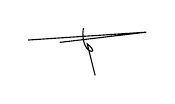
\begin{tikzpicture}\draw (0,0)--(1.5,.1)--(.4,-.03);\draw (.7,.15) .. controls (.65,-.2) and (.95,-.2) .. (.75,-.05)--(.85,-.45);\end{tikzpicture}}

Supposons maintenant que de plus, on se soit donné une section $s$ de $X\deleted{\unsure{_S}}$ sur $S$, ne rencontrant pas $X'$ (i.e. une section de $X-X'$ sur $S$). Son image par $j$ est alors une section de $P^1_S-(\infty)$, i.e. une section de $\underline O_S$, appelée \uline{l'invariant} de $(X,X',\deleted{\unsure{j}}s)$, soit \deleted{\unsure{j}} $\unsure{i|j}$.

Supposons que l'invariant $\unsure{j|i}$ ne prenne nulle part les valeurs $0,1$ i.e. soit inversible, ainsi que $\unsure{j|i}-1$. Alors son image inverse dans $P^1_S$ \deleted{\unsure{x}} de $p:S\to P^1_S$ définit un \deleted{section} \inserted{revêtement} \uline{galoisien} \uline{de} $S$, \uline{non ramifié}, \uline{de groupe} $\mathfrak S_3$, \deleted{\unsure{et}} \uline{et c'est celui qui définit} $X$. [\unsure{À déduire des formalismes|À déduire les formules}
\mspage{43}
